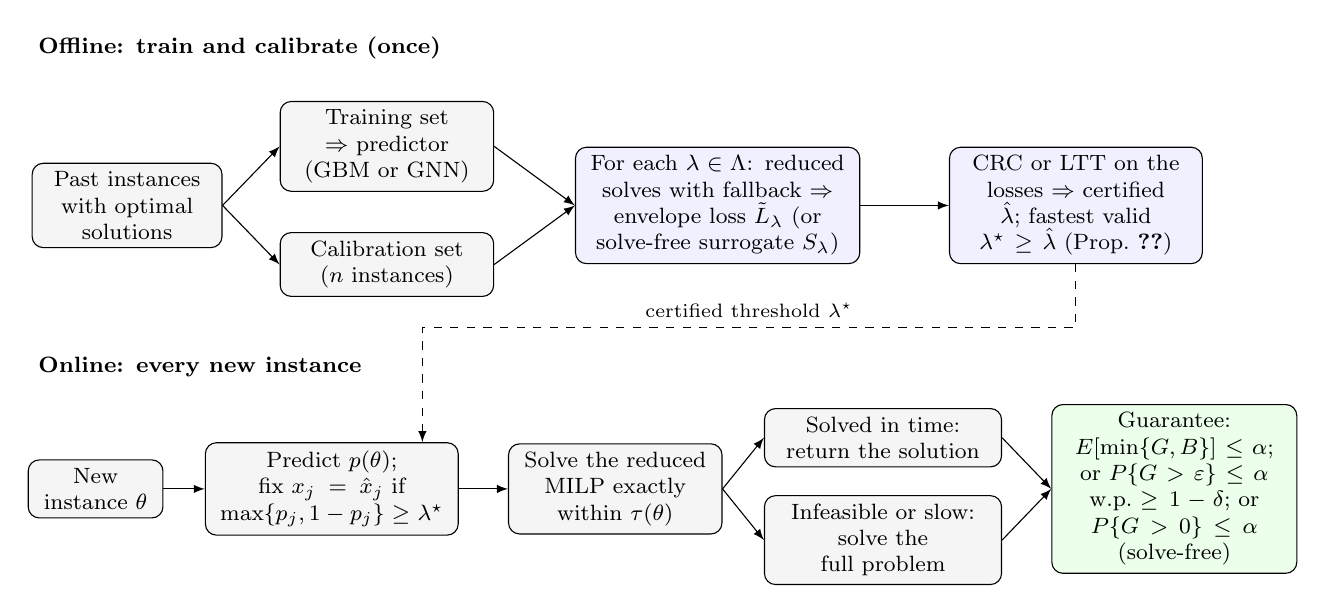
\begin{tikzpicture}[font=\footnotesize, >=latex,
  box/.style={draw, rounded corners, align=center, fill=gray!8, inner sep=3pt},
  par/.style={draw, rounded corners, align=center, fill=blue!6, inner sep=3pt},
  outb/.style={draw, rounded corners, align=center, fill=green!8, inner sep=3pt}]
 \node[anchor=west, font=\footnotesize\bfseries] at (0,2.0) {Offline: train and calibrate (once)};
 \node[box, text width=2.2cm] (past) at (1.25,0) {Past instances with optimal solutions};
 \node[box, text width=2.5cm] (train) at (4.55,0.75) {Training set $\Rightarrow$ predictor (GBM or GNN)};
 \node[box, text width=2.5cm] (cal) at (4.55,-0.75) {Calibration set\\ ($n$ instances)};
 \node[par, text width=3.4cm] (loss) at (8.75,0) {For each $\lambda\in\Lambda$: reduced solves with fallback $\Rightarrow$ envelope loss $\tilde L_\lambda$ (or solve-free surrogate $S_\lambda$)};
 \node[par, text width=3.0cm] (crc) at (13.3,0) {CRC or LTT on the losses $\Rightarrow$ certified $\hat\lambda$; fastest valid $\lambda^\star\ge\hat\lambda$ (Prop.~\ref{prop:fastest})};
 \draw[->] (past.east) -- (train.west); \draw[->] (past.east) -- (cal.west);
 \draw[->] (train.east) -- (loss.west); \draw[->] (cal.east) -- (loss.west);
 \draw[->] (loss) -- (crc);
 \node[anchor=west, font=\footnotesize\bfseries] at (0,-2.05) {Online: every new instance};
 \node[box, text width=1.5cm] (new) at (0.85,-3.6) {New\\ instance $\theta$};
 \node[box, text width=3.0cm] (pred) at (3.85,-3.6) {Predict $p(\theta)$; fix $x_j=\hat x_j$ if $\max\{p_j,1-p_j\}\ge\lambda^\star$};
 \node[box, text width=2.5cm] (solve) at (7.45,-3.6) {Solve the reduced MILP exactly within $\tau(\theta)$};
 \node[box, text width=2.8cm] (ok) at (10.85,-2.95) {Solved in time:\\ return the solution};
 \node[box, text width=2.8cm] (fb) at (10.85,-4.25) {Infeasible or slow:\\ solve the full problem};
 \node[outb, text width=2.9cm] (guar) at (14.55,-3.6) {Guarantee: $\mathbb{E}[\min\{G,B\}]\le\alpha$; or $\mathbb{P}\{G>\varepsilon\}\le\alpha$ w.p.\ $\ge1-\delta$; or $\mathbb{P}\{G>0\}\le\alpha$ (solve-free)};
 \draw[->] (new) -- (pred); \draw[->] (pred) -- (solve);
 \draw[->] (solve.east) -- (ok.west); \draw[->] (solve.east) -- (fb.west);
 \draw[->] (ok.east) -- (guar.west); \draw[->] (fb.east) -- (guar.west);
 \draw[->, dashed] (crc.south) -- (13.3,-1.55) -- node[above, font=\scriptsize, pos=0.5] {certified threshold $\lambda^\star$} (5.0,-1.55) -- (5.0,-3.6 |- pred.north);
\end{tikzpicture}
